\documentclass[12pt, a4paper, oneside]{ctexart}
\usepackage{amsmath, amsthm, amssymb, bm, color, framed, graphicx, hyperref, mathrsfs, float, caption}
\usepackage[justification=centering]{caption}

% multi-column
\usepackage{tasks}
% itemize
\NewTasksEnvironment[label=(\arabic*), label-width=3ex]{exercise}

\everymath{\displaystyle}

\title{\textbf{第五次作业}}
\author{U08M11002 Spring 2022}
\date{提交截止日期:北京时间2022年4月20日}
\linespread{1}
\definecolor{shadecolor}{RGB}{241, 241, 255}

\newcounter{problemname}
\newenvironment{problem}{\stepcounter{problemname}\par\noindent\textbf{题目\arabic{problemname}. }}{\\\par}
\newenvironment{warning}{\begin{shaded}\par\noindent\textbf{提交作业方式:}}{\end{shaded}\par}

\begin{document}
	
	\maketitle
	
	\begin{warning}
		具体提交方式请以 QQ 群里助教的通知为准。
		\begin{enumerate}
			\item 为了你自己复习需要,\textbf{建议上交前自行扫描备份}。
		\end{enumerate}
	\end{warning}
	
	\hspace{1em}
	
	
	\begin{problem}
		求下列函数的$F(jw)$:
		\begin{exercise}
			\task $f(t) = \frac{\sin2\pi(t-2)}{\pi(t-2)}$,$-\infty < t < \infty$;
			\task $f(t) = \frac{2a}{a^{2} + t^{2}}$,$-\infty < t < \infty$,$a > 0$;
			\task $f(t) = \Big(\frac{\sin2\pi t}{2\pi t}\Big)^{2}$,$-\infty < t < \infty$;
	\end{exercise}
		\quad
	\end{problem}
	
	
	\begin{problem}
		已知$f(t) = \frac{\sin t}{t}$,求其$F(jw)$,并证明
		$\int_{-\infty}^{\infty}\frac{\sin t}{t}\mathrm{dt} = \pi$。
		\quad
	\end{problem}
	
	\newpage
	
	\begin{problem}
		应用直接积分与傅里叶变换性质两种方法,求下图中所示余弦脉冲信号的傅里叶变换$F(jw)$。
		\begin{figure}[H]
			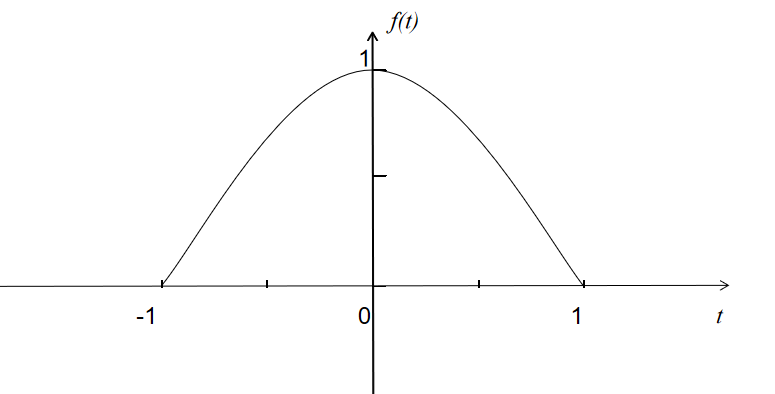
\includegraphics[width=10cm]{assets/hw5img1.png}
			\centering
		\end{figure}
		\quad
	\end{problem}
	
	
	\begin{problem}
		已知$f(t)$的傅里叶变换$F(jw)$,设$y(t) = f(\frac{t}{2} + 3) * \cos4t$,试求$y(t)$的傅里叶变换$Y(jw)$。
		\quad
	\end{problem}
	
	
	\begin{problem}
		已知$f(t) \Leftrightarrow F(jw)$,求下列信号的傅里叶变换:
		\begin{exercise}
			\task $y_1(t) = \frac{1}{2}f(t+1) + \frac{1}{2}f(t-1)$;
			\task $y_2(t) = f(-\frac{1}{2}t + 1) + f(\frac{1}{2}t - 1)$;
			\task $y_3(t) = f(t) \cdot \cos(\pi t)$;
			\task $y_4(t) = \frac{\sin3t}{t} * f(t)$;
			\task $y_5(t) = \frac{\mathrm{d} }{\mathrm{d} t}[f(-\frac{1}{4}t-1)]$;
		\end{exercise}
		\quad
	\end{problem}
	
	\newpage
	
	\begin{problem}
		求下列频谱函数的傅里叶逆变换:
		\begin{exercise}
			\task $F_1(jw) = 2\cos w$;
			\task $F_2(jw) = \frac{e^{j2w}}{jw + 1}$;
			\task $F_3(jw) = \frac{e^{-jw}}{6 - w^2 + 5jw}$;
		\end{exercise}
		\quad
	\end{problem}
	
	\begin{problem}
		已知$f(t) \Leftrightarrow F(jw)$,若$f_2(t) =\int_{-\infty}^{t} (t-2)f(4-2t) \mathrm{dt}$,求$f_2(t)$的傅里叶变换$F_2(jw)$。
		\quad
	\end{problem}
	
	\begin{problem}
		若已知$f(t) \Leftrightarrow F(jw)$,试求下列函数的频谱:
		\begin{exercise}(3)
			\task $tf(2t)$;
			\task $(t - 2)f(t)$;
			\task $t\frac{\mathrm{df(t)}}{\mathrm{dt}}$;
			\task $f(1 - t)$;
			\task $(1 - t)f(1 - t)$;
			\task $f(2t - 5)$;
			\task $\int_{-\infty}^{1 - \frac{1}{2}t} f(\tau) \mathrm{d\tau}$;
			\task $e^{jt}f(3 - 2t)$;
			\task $\frac{\mathrm{df(t)}}{\mathrm{dt}} * \frac{1}{\pi t}$;
		\end{exercise}
		\quad
	\end{problem}
    \begin{problem}
    	利用能量等式
    	$\int_{-\infty}^{\infty} f^2(t) \mathrm{dt} = \frac{1}{2\pi} \int_{-\infty}^{\infty} |F(jw)|^2 \mathrm{dw}$,计算下列积分的值:
    	\begin{exercise}
    		\task $\int_{-\infty}^{\infty} (\frac{\sin t}{t})^2 \mathrm{dt}$;
    		\task $\int_{-\infty}^{\infty} \frac{\mathrm{dx}}{(1+x^2)^2}$;
    	\end{exercise}
    \quad
    \end{problem}	
    
    \begin{problem}
    	已知信号$f(t)$的频谱函数$F(jw) = 4\mathrm{Sa}(w)\cos2w$,求信号$f(t)$。
    	\quad
    \end{problem}
	
\end{document}